\epi{我总是兴奋于阳光的轻抚和沉寂在早期编程语言中。
无需太多文字;许多已经完成了。
旧的程序阅读起来就像是同表达良好的研究工作者或受到良好训练的机器同事沟通一样,
而不是与编译器争论。谁愿意让其成熟到发出这样的声音呢?
}{\textsc{RICHARD P. GABRIEL}}

\noindent{}函数是构建 Go 程序的基础部件;所遇有趣的事情都是在它其中发生的。
函数的定义看起来像这样:
\begin{lstlisting}[caption=函数定义,label=src:function definition]
|\begin{tikzpicture}[overlay]
\ubrace{0.8,-1.5}{0.0,-1.5}{关键字~\key{func} 用于定义一个函数;}
%
\ubrace{2.9,-1.5}{0.9,-1.5}{函数可以绑定到特定的类型上。%
这叫做~\first{\emph{接收者}}{receiver}。有接收者的函数被称作%
~\index{方法}{method}。第~\ref{chap:interfaces} 章将对其进行说明;}
%
\ubrace{4.7,-1.5}{3.1,-1.5}{\emph{funcname} 是你函数的名字;}
%
\ubrace{6.1,-1.5}{4.9,-1.5}{\type{int} 类型的变量~\var{q} 作为输入参数。%
参数用~\first{\emph{pass-by-value}}{pass-by-value} 方式传递,意味着它们会被复制;}
%
\ubrace{8.1,-1.5}{6.4,-1.5}{%
变量~\var{r} 和~\var{s} 是这个函数的~\index{named return parameters}{命名返回值}。%
在~Go 的函数中可以返回多个值。参阅第~\pageref{sec:multiple return} 页的``\titleref{sec:multiple return}''。%
如果不想对返回的参数命名,只需要提供类型:\lstinline{(int,int)}。%
如果只有一个返回值,可以省略圆括号。如果函数是一个子过程,并且没有任何返回值,也可以省略这些内容;}
%
\ubrace{11.1,-1.5}{8.4,-1.5}{这是函数体。注意~\func{return} 是一个语句,所以包裹参数的括号是可选的。}
\end{tikzpicture}|
type mytype int	|\coderemark{新的类型,参阅第~\ref{chap:beyond} 章}|

func (p mytype) funcname(q int) (r,s int) { return 0,0 }
||
\end{lstlisting}

\showremarks
这里有两个例子,左边的函数没有返回值,右边的只是简单的将输入返回。

\begin{minipage}{.5\textwidth}
\begin{lstlisting}
func subroutine(in int) {
    return
}
\end{lstlisting}
\end{minipage}
\begin{minipage}{.5\textwidth}
\begin{lstlisting}
func identity(in int) int {
    return in
}
\end{lstlisting}
\end{minipage}

可以随意安排函数定义的顺序,编译器会在执行前扫描每个文件。所以函数原型在 Go 中都是过期的旧物。
Go 不允许函数嵌套。
然而你可以利用匿名函数实现它,参阅本章的 "\titleref{sec:functions as values}" 在
\pageref{sec:functions as values} 页。


递归函数跟其他语言是一样的:
\begin{lstlisting}[caption=递归函数]
func rec(i int) {
   if i == 10 {
        return
   }
   rec(i+1)
   fmt.Printf("%d ", i)
}
\end{lstlisting}
这会打印 \texttt{9 8 7 6 5 4 3 2 1 0}。

\section{作用域}
在 Go 中,定义在函数外的变量是\first{全局}{scope!local}的,
那些定义在函数内部的变量,对于函数来说是\first{局部}{scope!local}的。
如果命名覆盖——一个局部变量与一个全局变量有相同的名字——在函数执行的时候,
局部变量将覆盖全局变量。

\begin{minipage}{.5\textwidth}
\begin{lstlisting}[caption=局部作用域,label=src:scope1]
|\begin{tikzpicture}[overlay]
\draw [->,thick] (3.1,-5.00) arc (-60:90:2.00cm);
\draw [->,thick] (3.1,-7.00) arc (-60:90:0.20cm);
\end{tikzpicture}|
package main

var a = 6

func main() {
    p()
    q()
    p()
}

func p() {
    println(a)
}

func q() {
    a := 5|\coderemark{定义}|
    println(a)
}
\end{lstlisting}

\hfill
\vfill
\end{minipage}
\hfill
\begin{minipage}{.5\textwidth}
\begin{lstlisting}[caption=Global scope,label=src:scope2]
|\begin{tikzpicture}[overlay]
\draw [->,thick] (2.9,-5.00) arc (-60:90:2.00cm);
\draw [->,thick] (3.5,-7.00) arc (-60:90:3.15cm);
\end{tikzpicture}|
package main

var a = 6

func main() {
    p()
    q()
    p()
}

func p() {
    println(a)
}

func q() {
    a = 5|\coderemark{Assignment}|
    println(a)
}
\end{lstlisting}

\hfill
\vfill
\end{minipage}

在 \ref{src:scope1} 中定义了函数 \func{q()} 的局部变量 \var{a}。
局部变量 \var{a} 仅在 \func{q()} 中可见。这也就是为什么代码会打印:\texttt{656}。
在 \ref{src:scope2} 中没有定义局部变量,只有全局变量 \var{a}。
这将使得赋值全局可见。这段代码将会打印:\texttt{655}。

在下面的例子中,我们在 \func{f()} 中调用 \func{g()}:

\lstinputlisting[caption=当函数调用函数时的作用域]{src/scope3.go}

输出内容将是:\texttt{565}。\emph{局部}变量\emph{仅仅}在执行定义它的函数时有效。
%%Finally, one can create a \first{"function literal"}{function literal} in which you essentially 
%%define a function inside another
%%function, i.e. a \first{nested function}{nested function}. 
%%The following figure should clarify why it prints: \texttt{565757}. 
%%\begin{lstlisting}[caption=Scope and function literals,label=src:scope3,float]
|\begin{tikzpicture}[overlay]
\draw [->,thick] (2.8,-4.10) arc (-60:90:0.20cm);
\draw [->,thick] (2.8,-2.00) arc (-60:90:0.20cm);
\draw [->,thick] (2.4,-1.60) arc (-60:90:0.50cm);
%
\draw [->,thick] (4.4,-8.75) arc (-60:80:4.30cm);
% function f()
\draw [->,thick] (4.4,-5.85) arc (-60:90:0.30cm);
\draw [->,thick] (4.4,-5.25) arc (-60:90:0.90cm);
%
\draw [->,thick] (3.2,-7.45) arc (-60:65:2.00cm);
\end{tikzpicture}|
package main
var a int
func main() {
        a = 5
        println(a)
        f()
}
func f() {
        a := 6
        println(a)
        g()
        x := func() {
                a = 7
                println(a)
        }
        x()
        g()
        println(a)
}
func g() {
        println(a)
}
\end{lstlisting}


\section{Multiple return values}
\label{sec:multiple return}
One of Go's unusual features is that functions and methods can return multiple
values (Python can do this too). This can be used to improve on a couple of 
clumsy idioms in C programs:
in-band error returns (such as -1 for \texttt{EOF}) and modifying an argument.
In Go, \lstinline{Write} returns a count and an
error: "Yes, you wrote some bytes but not all of them because you filled the
device". The signature of \lstinline{*File.Write} in package
\package{os} is:
\begin{lstlisting}
func (file *File) Write(b []byte) (n int, err Error)
\end{lstlisting}
and as the documentation says, it returns the number of bytes written and a
non-\lstinline{nil} \var{Error} when \lstinline{n != len(b)}. This is a common
style in Go.

A similar approach obviates the need to pass a pointer to a return value to
simulate a reference parameter. Here's a simple-minded function to grab a
number from a position in a byte array, returning the number and the next
position.
\begin{lstlisting}
func nextInt(b []byte, i int) (int, int) {
    x := 0
    // Naively assume everything is a number
    for ; i < len(b); i++ {
        x = x*10 + int(b[i])-'0'
    }
    return x, i
}
\end{lstlisting}
You could use it to scan the numbers in an input array a like this:
\begin{lstlisting}
a := []byte{'1', '2', '3', '4'}
var x int
for i := 0; i < len(a); {	|\coderemark{No \texttt{i++}}|
    x, i = nextInt(a, i)
    println(x)
}
\end{lstlisting}
Without having tuples as a native type, multiple return values is the next
best thing to have. You can return precisely what you want without
overloading the domain space with special values to signal errors.

\section{Named result parameters}
\label{sec:named result parameters}
The return or result parameters of a Go function can be given names and used
as regular variables, just like the incoming parameters. When named, they are
initialized to the zero values for their types when the function begins; if the
function executes a \key{return} statement with no arguments, the current values of
the result parameters are used as the returned values. Using this
features enables you (again) to do more with less code \footnote{This is
a motto of Go; "Do \emph{more} with \emph{less} code".}.

The names are not mandatory but they can make code shorter and clearer:
\emph{they are documentation}. 
If we name the results of \lstinline{nextInt} it becomes obvious which
returned \type{int} is which.

\begin{lstlisting}
func nextInt(b []byte, pos int) (value, nextPos int) { /* ... */ }
\end{lstlisting}
Because named results are initialized and tied to an unadorned
\key{return},
they can simplify as well as clarify. Here's a version of
\lstinline{io.ReadFull} that uses them well:

\begin{lstlisting}
func ReadFull(r Reader, buf []byte) (n int, err os.Error) {
    for len(buf) > 0 && err == nil {
        var nr int
        nr, err = r.Read(buf)
        n += nr
        buf = buf[nr:len(buf)]
    }
    return
}
\end{lstlisting}
In the following example we declare a simple function which calculates
\gomarginpar{Some text in this section comes from \cite{go_intro}.}  % layout
the factorial value of a value \var{x}.
\begin{lstlisting}
func Factorial(x int) int { |\coderemark{\texttt{func Factorial(x int) (int)} is also OK}|
   if x == 0 {
      return 1
   } else {
      return x * Factorial(x - 1)
   }
}
\end{lstlisting}
So you could also write factorial as:
\begin{lstlisting}
func Factorial(x int) (result int) {
  if x == 0 {
    result = 1	
  } else {
    result = x * Factorial(x - 1)
  }
  return
}
\end{lstlisting}
When we use named result values, the code is shorter and
easier to read.
You can also write a function with multiple return values:
\begin{lstlisting}
func fib(n) (val, pos int) { |\coderemark{Both ints}|
   if n == 0 {
      val = 1
      pos = 0
   } else if n == 1 {
      val = 1
      pos = 1
   } else {
      v1, _ := fib(n-1)
      v2, _ := fib(n-2)
      val = v1 + v2
      pos = n
   }
   return
}
\end{lstlisting}

\section{Deferred code}
\label{sec:deferred code}
Suppose you have a function in which you open a file and perform various
writes and reads on it. In such a function there are often spots where
you want to return early. If you do that, you will need to close the file
descriptor you are working on. This often leads to the following code:
\begin{lstlisting}[caption=Without defer]
func ReadWrite() bool {
    file.Open("file")
    // Do your thing
    if failureX {
	file.Close()
	return false
    }

    if failureY {
	file.Close()
	return false
    }
    file.Close()
    return true
}
\end{lstlisting}
Here a lot of code is repeated. To overcome this Go has the
\first{\key{defer}}{keyword!defer} statement. After
\key{defer} you specify a function which is called just \emph{before} a
return from the function is executed.

The code above could be rewritten as follows. This makes the 
function more readable, shorter and puts the \func{Close} right next 
to the \func{Open}.
\begin{lstlisting}[caption=With defer]
func ReadWrite() bool {
    file.Open("file")
    defer file.Close()	|\coderemark{\func{file.Close()} \emph{is} the function}|
    // Do your thing
    if failureX {
	return false    |\coderemark{\func{Close()} is now done automatically}|
    }
    if failureY {
	return false    |\coderemark{And here too}|
    }
    return true
}
\end{lstlisting}
You can put multiple functions on the "deferred list"\index{deferred list}, like this
example from \cite{effective_go}:
\begin{lstlisting}
for i := 0; i < 5; i++ { 
    defer fmt.Printf("%d ", i) 
} 
\end{lstlisting}
Deferred functions are executed in LIFO order, so the above code
prints: \lstinline{4 3 2 1 0}. 

With \func{defer} you can even change return values, provided that
you are using named result parameters and a function
literal\index{function!literal}\footnote{A function literal
is sometimes called a \index{closure} closure.}, i.e:
\begin{lstlisting}[caption=Function literal]
defer func() {
	/* ... */
}()		 |\coderemark{() is needed here}|
\end{lstlisting}
Or this example which makes it easier to understand why and where
you need the braces:
\begin{lstlisting}[caption=Function literal with parameters]
defer func(x int) {
	/* ... */
}(5)		 |\coderemark{Give the input variable \var{x} the value 5}|
\end{lstlisting}
In that (unnamed) function you can access any named return
parameter:
\begin{lstlisting}[caption=Access return values within defer]
func f() (ret int) {    |\coderemark{\var{ret} is initialized with zero}|
	defer func() {
		ret++	|\coderemark{Increment \var{ret} with 1}|
	}()
	return 0	|\coderemark{1 \emph{not} 0 will be returned!}|
}
\end{lstlisting}

\section{Variadic parameters}
Functions that take variadic parameters are functions that have a
variable number of parameters. To do this, you first
need to declare your function to take variadic arguments:
\begin{lstlisting}
func myfunc(arg ...int) {}
\end{lstlisting}
The \lstinline{arg ... int} instructs Go to see this as a function that
takes a variable number of arguments. Note that these arguments all
have the type \type{int}. Inside your function's body the variable
\var{arg} is a slice of ints:
\begin{lstlisting}
for _, n := range arg {
    fmt.Printf("And the number is: %d\n", n)
}
\end{lstlisting}
If you don't specify the type of the variadic argument it defaults to the
empty interface \var{interface\{\}} (see chapter
\ref{chap:interfaces}").
Suppose we have another variadic function called \func{myfunc2}, the 
following example shows how to pass the variadic arguments to it:
\begin{lstlisting}
func myfunc(arg ...int) {
    myfunc2(arg...)  |\coderemark{Pass it as-is}|
    myfunc2(arg[:2]...)  |\coderemark{Slice it}|
}
\end{lstlisting}

\section{Functions as values}
\label{sec:functions as values}
\index{function!as values}
\index{function!literals}
As with almost everything in Go, functions are also \emph{just} values.
They can be assigned to variables as follows:
\lstinputlisting[label=src:anonfunc,caption=Anonymous function,linerange={3,}]{src/anon-func.go}
If we use \lstinline{fmt.Printf("%T\n", a)} to print the type of
\var{a}, it prints \func{func()}.

Functions--as--values may also be used in other places, like in maps.
Here we convert from integers to functions:
\begin{lstlisting}[caption=Functions as values in maps]
var xs = map[int]func() int{
    1: func() int { return 10 },
    2: func() int { return 20 },
    3: func() int { return 30 }, |\coderemark{Mandatory ,}|
    /* ... */
}
\end{lstlisting}
Or you can write a function that takes a function as its parameter, for
example a \func{Map} function that works on \type{int} slices. This is
left as an exercise for the reader, see exercise Q\ref{ex:map function}
on page \pageref{ex:map function}.

\section{Callbacks and closures}
\label{sec:callbacks}
With functions as values they are easy to pass to functions, from where
they can be used as callbacks. First define a function that
does "something" with an integer value:
\begin{lstlisting}
func printit(x int) {       |\coderemark{Function returns nothing}|
    fmt.Print("%v\n", x)    |\coderemark{Just print it}|

}
\end{lstlisting}
The signature of this function is: \lstinline{func printit(int)}, or
without the function name: \mbox{\lstinline{func(int)}}. To create a new function
that uses this one as a callback we need to use this signature:
\begin{lstlisting}
func callback(y int, f func(int)) { |\coderemark{\func{f} will hold the function}|
    f(y)    |\coderemark{Call the callback \func{f} with \var{y}}|
}
\end{lstlisting}
We've already seen some use of closures in section "\titleref{sec:deferred code}", but there
is more to tell. When you define a closure, i.e. when you start using a function
literal you still have access to the (local) variables defined in the current
function.

\begin{lstlisting}
// Define some local vars
// This code is WAY to complex, but illustrates it nicely
    frameSquare := func(x, y int) {
            // closure effortlessly passes local variables to callback
            if thickFrame {
                    // draw 3 x 3 pixel block for thicker rectangle
                    for x0 := x - 1; x0 <= x+1; x0++ {
                            for y0 := y - 1; y0 <= y+1; y0++ {
                                    rgba.Set(x0, y0, redColor)
                            }
                    }
            } else {
                    rgba.Set(x, y, blueColor)
            }
    }
\end{lstlisting}

If you want to do this by \emph{not} using a closure and defining a completely new
function you need to pass all vars to the function.
\todo{Gist is there, but needs much better wording and code}



\section{Panic and recovering}
\label{sec:panic}
Go does not have a exception mechanism, like that in Java for instance: you can not throw exceptions.
Instead it using a panic-and-recover mechanism. It is worth remembering that you should use this as
a last resort, your code will not look, or be, better if it is littered with panics. It's a powerful tool:
use it wisely. So, how do you use it.

The following description was taken from \cite{go_blog_panic}:
\begin{description}
\item[Panic]{is a built-in function that stops the ordinary flow of control and begins panicking. When the function 
\func{F} calls \key{panic},
execution of \func{F} stops, any deferred functions in \func{F} are executed normally, and 
then \func{F} returns to its caller. To the caller, \func{F} then
behaves like a call to \key{panic}. The process continues up the stack until all functions in the current 
goroutine have returned, at which point the program crashes. 

Panics can be initiated by invoking \func{panic} directly. They can also be caused by \emph{runtime errors}, such
as out-of-bounds array accesses.}

\item[Recover]{is a built-in function that regains control of a panicking goroutine. Recover is \emph{only} useful inside 
\emph{deferred} functions.

During normal execution, a call to \func{recover} will return \type{nil} and have no other effect. 
If the current goroutine is panicking, a call
to \func{recover} will capture the value given to \func{panic} and resume normal execution.}
\end{description}

\section{Exercises}
\begin{Exercise}[title={平均值},difficulty=4]
\label{ex:average}
\Question\label{ex:average q1} 编写一个函数用于计算一个 \type{float64} 类型的 slice 的平均值。
\end{Exercise}

\begin{Answer}
\Question 下面的函数计算平均值。
\lstinputlisting[caption=Go 中的平均值函数,linerange={3,14}]{ex-functions/src/ave.go}
\showremarks
\end{Answer}


\begin{Exercise}[title={整数顺序},difficulty=3]
\label{ex:ordering function}
\Question 编写函数,返回其(两个)参数正确的(自然)数字顺序:
\newline 
\lstinline{f(7,2)} $\rightarrow$ \lstinline{2,7}\newline
\lstinline{f(2,7)} $\rightarrow$ \lstinline{2,7}\newline
\end{Exercise}

\begin{Answer}
\Question 
这里可以利用~Go 中的多返回值(参阅``\titleref{sec:multiple return}''小节):
\begin{lstlisting}
func order(a, b int) (int, int) {
        if a > b { 
                return b,a 
        }   
        return a,b 
}
\end{lstlisting}

\end{Answer}


\begin{Exercise}[title={作用域},difficulty=4]
\label{ex:scope}
\Question\label{ex:scope q1} 下面的程序有什么错误?

\begin{lstlisting}[numbers=right]
package main

import "fmt"
                                                                                                   
func main() {
        for i := 0; i < 10; i++ {
                fmt.Printf("%v\n", i)
        }
	fmt.Printf("%v\n", i)
}
\end{lstlisting}

\end{Exercise}

\begin{Answer}
\Question
这个程序不能被编译,由于第 9 行的变量 \var{i},未定义:
\var{i} 仅在 \key{for} 循环中有效。为了修正这个,
\func{main()} 应修改为:
\begin{lstlisting}[numbers=none]
func main() {
        var i int
        for i = 0; i < 10; i++ {
                fmt.Printf("%v\n", i)
        }
	fmt.Printf("%v\n", i)
}
\end{lstlisting}
现在 \var{i} 在 \key{for} 循环外定义,并且在其后仍然可访问。
这会打印数字从 0 到 10。
\end{Answer}


\begin{Exercise}[title={Stack},difficulty=5]
\label{ex:stack}
\Question \label{ex:stack q1} Create a simple stack which can hold a
fixed amount of ints. It does not have to grow beyond this limit.
Define both a \func{push} -- put something on the stack -- and a \func{pop} 
-- retrieve something from the stack -- function. The stack should be
a LIFO (last in, first out) stack.

\begin{figure}[H]
\caption{A simple LIFO stack}
\label{fig:stack}
\begin{center}
\includegraphics[scale=0.65]{fig/stack.pdf}
\end{center}
\end{figure}

\Question \label{ex:stack q2} Bonus. Write a \func{String} method which 
converts the stack to a string representation.  This way you can print the stack using:
\lstinline{fmt.Printf("My stack %v\n", stack)}

\noindent{}The stack in the figure could be represented as:
\texttt{[0:m] [1:l] [2:k]}

\end{Exercise}

\begin{Answer}

\Question 
%%\subsection*{Define our type} maybe nice to do this
First we define a new type that represents a stack; we need an
array (to hold the keys) and an index, which points to the last element.
Our small stack can only hold 10 elements.

\begin{lstlisting}
type stack struct { |\coderemark{\emph{stack} is not exported}|
    i    int 
    data [10]int  
}
\end{lstlisting}

Next we need the \func{push} and \func{pop} functions to actually
use the thing. \emph{First we show the \emph{wrong}{} solution!}
In Go data passed to functions is \emph{passed-by-value} meaning a copy
is created and given to the function. The first stab for the function
\func{push} could be:

\begin{lstlisting}
func (s stack) push(k int) { |\coderemark{Works on copy of argument}|
	if s.i+1 > 9 {
		return
	}
	s.data[s.i] = k
	s.i++
}
\end{lstlisting}
The function works on the \var{s} which is of the type \type{stack}. To
use this we just call \lstinline{s.push(50)}, to push the integer 50 on
the stack. But the push function gets a copy of \var{s}, so it is
\emph{not} working the \emph{real} thing. Nothing gets pushed to our
stack this way, for example the following code:

\begin{lstlisting}
var s stack |\coderemark{make \var{s} a simple \type{stack} variable}|
s.push(25)
fmt.Printf("stack %v\n", s);
s.push(14)
fmt.Printf("stack %v\n", s);
\end{lstlisting}
prints:
\vskip\baselineskip
\begin{display}
stack [0:0]
stack [0:0]
\end{display}
\vskip\baselineskip

To solve this we need to give the function \func{push} a pointer
to the stack. This means we need to change \func{push} from

\lstinline{func (s stack) push(k int)} 
$\rightarrow$
\lstinline{func (s *stack) push(k int)}

We should now use \func{new()} (see ``\titleref{sec:allocation with new}''
in chapter \ref{chap:beyond}) to create a \emph{pointer} to a newly
allocated \type{stack}, so line 1 from the example above needs to be
\lstinline{s := new(stack)}

\noindent{}And our two functions become:
\begin{lstlisting}
func (s *stack) push(k int) {
	s.data[s.i] = k
	s.i++
}

func (s *stack) pop() int {
	s.i--
	return s.data[s.i]
}
\end{lstlisting}
Which we then use as follows
\begin{lstlisting}
func main() {
	var s stack
	s.push(25)
	s.push(14)
	fmt.Printf("stack %v\n", s)
}
\end{lstlisting}

\Question While this was a bonus question, having the ability to print
the stack was very valuable when writing the code for this exercise.
According to the Go documentation \lstinline{fmt.Printf("%v")} can
print any value (\%v) that satisfies the \func{Stringer} interface.
For this to work we only need to define a \func{String()} function for
our type:
\begin{lstlisting}[caption=stack.String()]
func (s stack) String() string {
	var str string
	for i := 0; i <= s.i; i++ {
		str = str + "[" +
			strconv.Itoa(i) + ":" + strconv.Itoa(s.data[i]) + "]"
	}
	return str
}
\end{lstlisting}
\end{Answer}


\begin{Exercise}[title={变参},difficulty=5]
\label{ex:varargs}
\Question\label{ex:varargs q1}
编写函数接受整数类型变参,并且每行打印一个数字。
\end{Exercise}

\begin{Answer}
\Question
需要使用 \lstinline{...} 语法来实现函数接受若干个数字作为变参。

\lstinputlisting[label=src:varargs,caption=有变参的函数]{ex-functions/src/var-arg.go}

\end{Answer}


\begin{Exercise}[title={斐波那契},difficulty=5]
\label{ex:fibonaci}
\Question\label{ex:fibonaci q1}
斐波那契数列以:$1, 1, 2, 3, 5, 8, 13, \ldots$ 开始。
或者用数学形式表达:$ x_1 = 1; x_2 = 1; x_n = x_{n-1} +
x_{n-2}\quad\forall n > 2 $。

编写一个接受~\type{int} 值的函数,并给出这个值得到的斐波那契数列。

\end{Exercise}

\begin{Answer}
\Question
下面的程序会计算出斐波那契数列。
\lstinputlisting[label=src:fib,caption=Go 编写的斐波那契函数]{ex-functions/src/fib.go}

\showremarks
\end{Answer}


\begin{Exercise}[title={Map function},difficulty=4]
\label{ex:map function}
\func{map()} 函数是一个接受一个函数和一个列表作为参数的函数。
函数应用于列表中的每个元素,而一个新的包含有计算结果的列表被返回。
因此: 
$$ map(f(), (a_1,a_2,\ldots,a_{n-1},a_n)) =  (f(a_1), f(a_2),\ldots,f(a_{n-1}), f(a_n)) $$
\Question \label{ex:map function q1} 编写 Go 中的简单的 \func{map()} 函数。
它能工作于操作整数的函数就可以了。
\Question \label{ex:map function q2} 扩展代码使其工作于字符串列表。

\end{Exercise}

\begin{Answer}

\Question 
\begin{lstlisting}[caption=Map 函数]
func Map(f func(int) int, l []int) []int {
        j := make([]int, len(l))
        for k, v := range l {
                j[k] = f(v)
        }
        return j
}

func main() {
        m := []int{1, 3, 4}
        f := func(i int) int {
                return i * i
        }
        fmt.Printf("%v", (Map(f, m)))
}
\end{lstlisting}

\Question 字符串问题的答案
\end{Answer}




\begin{Exercise}[title={Minimum and maximum},difficulty=3]
\label{ex:minmax}
\Question\label{ex:minmax q1} Write a function that calculates the
maximum value in an \type{int} slice (\type{[]int}).

\Question\label{ex:minmax q2} Write a function that calculates the
minimum value in a \type{int} slice (\type{[]int}).

\end{Exercise}

\begin{Answer}
\Question This a function for calculating a maximum:
\begin{lstlisting}
func max(l []int) (max int) {   |\longremark{We use a named return parameter;}|
        max = l[0]      
        for _, v := range l {   |\longremark{Loop over \var{l}. The index of the element is %
not important;}|
                if v > max {    |\longremark{If we find a new maximum, remember it;}|
                        max = v 
                }   
        }   
        return  |\longremark{A ``lone'' return, the current value of \var{max} is now returned.}|
}
\end{lstlisting}
\showremarks

\Question This a function for calculating a minimum, that is almost identical to \func{max}:
\begin{lstlisting}
func min(l []int) (min int) {
        min = l[0]
        for _, v := range l { 
                if v < min {
                        min = v 
                }   
        }   
        return
}
\end{lstlisting}
The interested reader may combine \func{max} and \func{min} into one function with a selector
that lets you choose between the minimum or the maximum, or one that returns both values.
\end{Answer}


\begin{Exercise}[title={冒泡排序},difficulty=1]
\label{ex:bubble}
\Question\label{ex:bubble q1} 编写一个针对~int 类型的~slice 冒泡排序的函数。这里 \cite{bubblesort}:
\begin{quote}
它在一个列表上重复步骤来排序,比较每个相邻的元素,并且顺序错误的时候,交换它们。
一遍一遍扫描列表,直到没有交换为止,这意味着列表排序完成。
算法得名于更小的元素就像``泡泡''一样冒到列表的顶端。
\end{quote}

\cite{bubblesort} 这里有一个过程代码作为示例:
\begin{lstlisting}[language=pascal]
procedure bubbleSort( A : list of sortable items )
  do
    swapped = false
    for each i in 1 to length(A) - 1 inclusive do:
      if A[i-1] > A[i] then
        swap( A[i-1], A[i] )
        swapped = true
      end if
    end for
  while swapped
end procedure
\end{lstlisting}
\end{Exercise}

\begin{Answer}
\Question 
冒泡排序并不是最有效率的,对于~$n$ 个元素它的算法复杂度是~$O(n^2)$。
快速排序~\cite{quicksort} 是更好的排序算法。

但是冒泡排序容易实现。
\lstinputlisting[caption=冒泡排序,linerange=4-19]{ex-functions/src/bubblesort.go}

由于~slice 是一个引用类型,\func{bubblesort} 函数可以工作,并且无须返回排序后的~slice。
\end{Answer}


\begin{Exercise}[title={函数返回一个函数},difficulty=6]
\label{ex:function}
\Question\label{ex:function q1} 编写一个函数返回另一个函数,返回的函数的作用是对一个整数~$+2$。
函数的名称叫做~\func{plusTwo}。
然后可以像下面这样使用:
\begin{lstlisting}
p := plusTwo()
fmt.Printf("%v\n", p(2))
\end{lstlisting}
应该打印 4。
参阅第~\pageref{sec:callbacks} 页的~``\titleref{sec:callbacks}''小节了解更多相关信息。

\Question\label{ex:function q2} 使~\ref{ex:function q1} 中的函数更加通用化,
创建一个~\func{plusX(x)} 函数,返回一个函数用于对整数加上~\var{x}。
\end{Exercise}

\begin{Answer}
\Question
\begin{lstlisting}
func main() {
        p2 := plusTwo()
        fmt.Printf("%v\n",p2(2))
}

func plusTwo() func(int) int { |\longremark{定义新的函数返回一个函数。%
看看你写的跟要表达的意思是如何的;}|
        return func(x int) int { return x + 2 } |\longremark{函数符号,%
在返回语句中定义了一个~+2 的函数。}|
}
\end{lstlisting}
\showremarks

\Question
这里我们使用闭包:
\begin{lstlisting}
func plusX(x int) func(int) int { |\longremark{再次定义一个函数返回一个函数;}|
        return func(y int) int { return x + y } |\longremark{在函数符号中使用\emph{局部}变量 \var{x}。}|
}
\end{lstlisting}
\showremarks
\end{Answer}


\cleardoublepage
\section{Answers}
\shipoutAnswer
